\section{Simplicial complexes and polyhedra}

Our aim is to create a good environment to prove an analogon of the Goldblatt-Thomason theorem for polyhedral semantics.

Let's begin by setting the objects we are going to find interplay between:
\subsection{Simplicial complexes geometrically and combinatorially}

Intuitively, any polygon can be obtained by gluing together triangles on their edges or vertices. Similarly we can describe a polyhedron 
as a gluing of simplices (higher dimensional triangles):

\begin{definition}[Geometric Simplex]\hfill 

    The \textbf{standard n-simplex} in $\R^{n+1}$ is the set 
    \[\Delta^n=\set{x\in\R^{n+1}:x_0+...+x_n=1,\ x_i\geq 0\text{ for }i=0,...,n}\]
    endowed with the topology induced by $\R^{n+1}$. 
    
    Note that every standard n-simplex comes equipped with $n+1$ 'canonical' subsimplices, those given by 
    the intersection with the canonical hyperplanes:
    \[\Delta^n\geq\Delta^{n-1}_i=\set{x\in\R^{n+1}:x_0+...+\hat{x_i}+...+x_n=1,\ x_i\geq 0\text{ for }i=0,...,n}\footnote{here the hat means 'that component is removed'.}\]
    We call such subsimplices and all their such subsimplices \textbf{faces} of $\Delta^n$

    We call an \textbf{n-simplex} in $\R^m$ an affine immersion $\Delta^n\hookrightarrow\R^m$, i.e. (the image of) an affine map
    \[j(\vec{x})= A\vec{x}+q:\R^{n+1}\to\R^m\] restricted to the simplex.
\end{definition}

With this definition, we have what we expect:
a 0-simplex is a point, a 1-simplex is a segment, a 2-simplex is a triangle, etc.

We can obtain a polyhedra by gluing together simplices: 
\begin{definition}[Polyhedron]\hfill 

    A \textbf{(Geometric) simplicial complex} is a collection $K$ of simplices in $\R^m$ such that 
    \begin{enumerate}
        \item Every face of a simplex in $K$ is in $K$, 
        \item The intersection of two simplices of $K$ is either empty or a face of both simplices.
    \end{enumerate}
    
    We call a \textbf{Polyhedron} in $\R^m$ the union of all elements of a geometric simplicial complex.

    If $K$ is a simplicial complex we call $|K|$ its \textbf{realization}, i.e. its associated polyhedron,
    and given a polyhedron $P$, any simplicial complex $K$ such that $|K|=P$ is called a \textbf{triangulation} of $P$.

    The topology we consider is the so called \textbf{Weak} topology, i.e. the one generated by the opens of all the faces contained
    in it.
\end{definition}

\begin{lemma}

    If $K$ is finite, then $|K|$ is compact
\end{lemma}
\begin{proof}
    It's a closed and bounded subset of $\R^n$.
\end{proof}

We make polyhedra into a category via $\PL-$homeomorphisms: We consider maps that are affine when restricted to any face.
More details can be found at \cite{PLTopology} or (closer to the aim of the paper \cite{DBLP}, \cite{TENCATE})

We may notice that a simplex is uniquely determined by its vertices, and a simplicial complex is uniquely determined 
by its simplices.

This means that we can give an abstract definition
\begin{definition}[Simplicial Complex]\hfill 

    A \textbf{(Combinatorial) simplicial complex}\footnote{The standard nomenclature is 
    \textbf{Abstract simplicial complex}: I found that "combinatorial" fit the description better and created 
    a more interesting duality with the geometric counterpart} is a collection of finite sets $K$ called \textbf{simplices}, that is closed under taking subsets, or 
    equivalently, is a set of vertices $V$ together with a collection $K\subseteq \Pp(V)$ (once again, of \textbf{simplices}), closed under taking subsets.   

    We make simplicial complexes into a category by saying that a map of simplicial complexes is a function $V\to V'$ such that the image of any simplex is a simplex.
\end{definition}

\begin{lemma} Every geometric simplicial complex uniquely determines a combinatorial simplicial complex
\end{lemma}
\begin{proof}

    Let $K$ be a geometric simplicial complex. Construct $K^v$ by sending each simplex in $K$ to the set of vertices of $K$.
    
    This is a combinatorial simplicial complex, since if $\set{v_1,...,v_n}\in K^v$ and $\set{w_1,...,w_k}\subseteq \set{v_1,...,v_n}$, then 
    $\set{w_1,...,w_k}$ are the vertices of a face of $K$, thus an element of $K^v$.
\end{proof}

\begin{lemma} Every finite combinatorial simplicial complex determines a geometric simplicial complex up to PL-isomorphism.
\end{lemma}
\begin{proof}
    We can realize every simplex to the standard simplex of the correct dimension, then glue them according to the data of the simplicial complex:

    \[\tilde{K}=\dfrac{\bigsqcup_{\sigma\in K}\Delta^{|\sigma|}}{\sim}\]

    Where $\Delta_i\sim\Delta_j$ if they correspond to the same simplex in $K$.

    The realization of this complex only depends on the immersion of its faces, thus any two will be isomorphic, and the total map will be affine when restricted
    to the faces, thus $PL$.
\end{proof}

From now on we refer to "combinatorial simplicial complexes" as just "simplicial complexes".

The previous lemmas mean that we have a correspondence
\[\set{\text{Simplicial complexes}}\rightarrow \set{\text{Polyhedra}}\]

We can extend it to a functor by noticing that 
\begin{lemma}
    Every simplicial map $K\to K'$ induces a PL map $|K|\to|K'|$
\end{lemma}
\begin{proof}[sketch of proof]
    Notice that every morphism of simplices can be realized as an affine map between their realizations.
\end{proof}

Thus we have what is commonly known as the realization:
\begin{definition}[Realization Functor]
    Call $\Scplx$ the category of simplicial complexes and $\Pol$ the category of polyhedra described above,
    We call the functor realizing a simplicial complex into a polyhedron 
    \[|-|:\Scplx\to\Pol\]
    The \textbf{realization functor}.
\end{definition}

\subsection{The face poset and nerves.}

Notice that any simplicial complex comes equipped with a 'face' order:

\begin{definition}[Face poset]\hfill

    Let $\Sigma$ be a simplicial complex. Then 
    \begin{itemize}
    \item $(\Sigma,\subseteq)$ is a poset, that we call the \textbf{Face poset} of $\Sigma$ and we denote $[\Sigma]$%^\text{op}$
    %\item $(\Sigma,\supseteq)$ is a poset, that we call the \textbf{Coface poset of} $\Sigma$ and we denote $[\Sigma]$\footnote{the reason for this notation will become clearer later.}
    \end{itemize}
\end{definition}

Note that every morphism of simplicial complexes induces a morphism of the posets -i.e. a monotone map- by taking the image of the function.
It's easy to check that we have a "sort of forgetful" functor 
\[[-]:\Scplx\to \Pos\]

As a 'forgetful' we expect there to exist a functor in the other direction that 'freely' generates a simplicial complex 
expressing the information of the poset; indeed

\begin{definition}[Nerve of a poset]\hfill 

    Let $(P,\leq)$ be a poset. The \textbf{Nerve} $\Nn(P)$ is a simplicial complex constructed in the following way:
    \begin{itemize}
        \item  The \textbf{vertices} are the points of $P$.
        \item  The \textbf{sides} are the $1$-chains $p_0\leq p_1$ in $P$.
        \item  The \textbf{Triangles} are the $2-$chains $p_0\leq p_1\leq p_2$ in $P$.
        \item  $\vdots $
        \item The \textbf{n-simplices} are the $n-$chains $p_0\leq p_1\leq\cdots\leq p_n$ in $P$.
        \item $\vdots$
    \end{itemize}

    This is clearly a simplicial complex as for any $m<n$, any sub-$m$-chain on an $n-$chain is part of the complex.

    On morphisms $\N$ acts like the direct image:

    Given a monotone map $f:(P,\leq)\to (Q,\leq)$, if $p_0\leq...\leq p_k$ is a simplex in $P$, $f(p_0)\leq...\leq f(p_k)$ 
    for monotonicity is a chain, thus a simplex in $Q$.
\end{definition}

This is clearly not an inverse of $[-]$: $\Nn[\Sigma]$ generally has more points than $\Sigma$.

Let's talk of a way we can recover information from the nerve process.

\subsection{Subdivisions}
\begin{definition}[Stellar moves]\hfill 

    Given two disjoint simplicial complexes $\Sigma$ and $\Sigma'$ we define:
    
    \noindent Their \textbf{join} $\Sigma\vee\Sigma'$ to be 
    \[\set{\sigma\cup\sigma': \sigma\in\Sigma,\sigma'\in\Sigma'}\]
    The \textbf{Star} of a face $\sigma$ to be 
    \[\bigstar_\Sigma(\sigma)\coloneq\set{\tau\in\Sigma:\tau\cup\sigma\in\Sigma}\]
    The \textbf{link} of a face $\sigma$ to be 
    \[\ell_\Sigma(\sigma)\coloneq \set{\tau\in\bigstar_\Sigma(\sigma): \tau\cap\sigma=\emptyset}\]
    Lastly, the \textbf{deletion} of a face $\sigma$ as 
    \[\Sigma\setminus\sigma\coloneq \set{\tau\in\Sigma: \sigma\not{\subseteq}\tau}\]
    and the \textbf{boundary} of a face $\sigma$ as 
    \[\partial\sigma=\set{\tau\in \Sigma: \tau\subsetneq \sigma}\]
    
    \noindent A \textbf{stellar subdivision} of a complex $\Sigma$ at $\sigma$ is a simplicial complex 
    \[(\Sigma\setminus\sigma) \cup (\set{x}\vee\partial \sigma\vee \ell_\Sigma(\sigma))\]
    where $x$ is a new vertex we are introducing.
    
    We call a \textbf{stellar move} of a complex either a stellar subdivision or its inverse, and we say that 
    two complexes are \textbf{stellarly equivalent} $\Sigma\sim_\star\Sigma'$ if there exist a complex $\Sigma''$ that can be obtained
    by $\Sigma$ or $\Sigma'$ via a sequence of stellar moves.
    \end{definition}
    
    \begin{theorem}[Alexander]\hfill 
    
    Two simplicial complexes are stellarly equivalent if and only if their geometric realizations are $\PL$-homeomorphic.    
    \end{theorem}
    \begin{proof}
        \cite{PLTopology}
    \end{proof}

    Also, a theorem that is of interest for us:
    \begin{theorem}\hfill 

    Stellarly equivalent simplicial complexes have bisimilar face posets.        
    \end{theorem}
    \begin{proof}\hfill

        A complete account can be found in \cite{Dekker}:

        A brief recap is that given a simplicial complex $\Sigma$ and $\Sigma_\sigma$ a subdivision of $\Sigma$ at a face $\sigma$, 
        there exists a unique $p-$morphism $[\Sigma_\sigma]\to[\Sigma]$, i.e. the morphism sending any face $s\in \Sigma_\sigma$
         to the smallest face of $\Sigma$ containing $s$.

        Here it is visually.
        \begin{figure}[H]
        \centering
        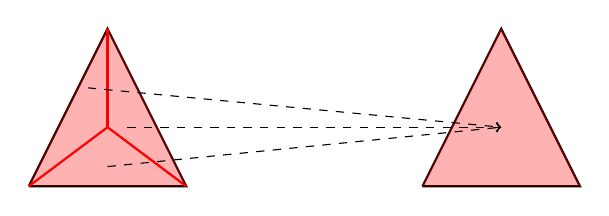
\begin{tikzpicture}
            \draw[thick] (-1,0)--(1,0)--(0,2)--(-1,0);
            \draw[red,thick](-1,0)--(0,0.75);
            \draw[red,thick](1,0)--(0,0.75);
            \draw[red,thick](0,2)--(0,0.75);
            \draw[red, opacity=0.3,fill](-1,0)--(0,2)--(1,0);
            \draw[thick] (4,0)--(6,0)--(5,2)--(4,0);
            \draw[red, opacity=0.3,fill](4,0)--(5,2)--(6,0);
            \draw[-to,dashed] (0,0.25)--(5,0.75);
            \draw[-to,dashed] (-0.25,1.25)--(5,0.75);
            \draw[-to,dashed] (0.25,0.75)--(5,0.75);
        \end{tikzpicture}
        \caption{A visual representation of the subdivision morphism acting on the polyhedron}
    \end{figure}
        Or, as posets 
        \begin{figure}[H]
        \centering            
    \begin{tikzcd}[ampersand replacement=\&,cramped]
	\& \textcolor{rgb,255:red,214;green,92;blue,92}{abx} \& \textcolor{rgb,255:red,214;green,92;blue,92}{bcx} \& \textcolor{rgb,255:red,214;green,92;blue,92}{acx} \&\&\&\&\& \textcolor{rgb,255:red,214;green,92;blue,92}{abc} \\
	ab \& ac \& bc \& \textcolor{rgb,255:red,214;green,92;blue,92}{ax} \& \textcolor{rgb,255:red,214;green,92;blue,92}{bx} \& \textcolor{rgb,255:red,214;green,92;blue,92}{cx} \&\& ab \& bc \& ac \\
	\& a \& b \& c \& \textcolor{rgb,255:red,214;green,92;blue,92}{x} \&\&\& a \& b \& c
	\arrow[no head, from=2-1, to=1-2]
	\arrow[no head, from=2-2, to=1-4]
	\arrow[no head, from=2-3, to=1-3]
	\arrow[no head, from=2-4, to=1-2]
	\arrow[no head, from=2-4, to=1-4]
	\arrow[no head, from=2-5, to=1-2]
	\arrow[no head, from=2-5, to=1-3]
	\arrow[no head, from=2-6, to=1-3]
	\arrow[no head, from=2-6, to=1-4]
	\arrow[from=2-6, to=2-8]
	\arrow[no head, from=2-8, to=1-9]
	\arrow[no head, from=2-9, to=1-9]
	\arrow[no head, from=2-10, to=1-9]
	\arrow[no head, from=3-2, to=2-1]
	\arrow[no head, from=3-2, to=2-2]
	\arrow[no head, from=3-2, to=2-4]
	\arrow[no head, from=3-3, to=2-1]
	\arrow[no head, from=3-3, to=2-3]
	\arrow[no head, from=3-3, to=2-5]
	\arrow[no head, from=3-4, to=2-2]
	\arrow[no head, from=3-4, to=2-3]
	\arrow[no head, from=3-4, to=2-6]
	\arrow[no head, from=3-5, to=2-4]
	\arrow[no head, from=3-5, to=2-5]
	\arrow[no head, from=3-5, to=2-6]
	\arrow[no head, from=3-8, to=2-8]
	\arrow[no head, from=3-8, to=2-10]
	\arrow[no head, from=3-9, to=2-8]
	\arrow[no head, from=3-9, to=2-9]
	\arrow[no head, from=3-10, to=2-9]
	\arrow[no head, from=3-10, to=2-10]
\end{tikzcd}
\caption{A visual representation of the subdivision morphism acting on the face poset}
\end{figure}

        Therefore if two simplicial complexes $\Sigma$ and $\Sigma'$ have a common subdivision $\Sigma''$, then 
        there exists a $p-$morphism $p_1:[\Sigma'']\to[\Sigma]$ and a $p-$morphism $p_2:[\Sigma'']\to[\Sigma']$.

        This means that we have a span of $p-$morphisms $[\Sigma]\gets[\Sigma'']\to[\Sigma']$, as any span of $p-$
        morphisms defines a bisimulation, we have that $[\Sigma]\leftrightarroweq[\Sigma']$.
    \end{proof}

Moreover, 
\begin{theorem}[Nerve]\hfill 

Let $\Sigma$ be a simplicial complex. then $\Nn([\Sigma])$ is a subdivision (the baricentric subdivision) of $\Sigma$.
\end{theorem}
\begin{proof}
    This is a well known fact that can be found in \cite{PLTopology}, among other sources.
\end{proof}    

\begin{figure}[H]
    \centering
    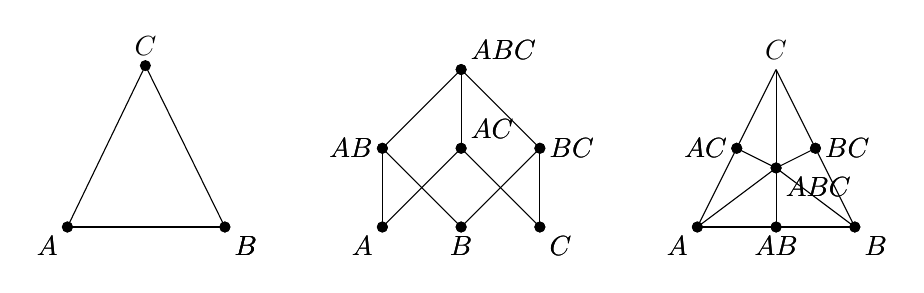
\begin{tikzpicture}[scale=1]
    % Coordinates
    \coordinate (A) at (-2.00, 0.00);
    \coordinate (B) at (-0.00, -0.00);
    \coordinate (C) at (-1.01, 2.05);
    \coordinate (D) at (2.00, 0.00);
    \coordinate (E) at (3.00, 0.00);
    \coordinate (F) at (4.00, 0.00);
    \coordinate (G) at (2.00, 1.00);
    \coordinate (H) at (3.00, 1.00);
    \coordinate (I) at (4.00, 1.00);
    \coordinate (J) at (3.00, 2.00);
    \coordinate (K) at (6.00, 0.00);
    \coordinate (L) at (8.00, 0.00);
    \coordinate (M) at (7.00, 2.00);
    \coordinate (N) at (6.50, 1.00);
    \coordinate (O) at (7.50, 1.00);
    \coordinate (P) at (7.00, 0.00);
    \coordinate (Q) at (7.00, 0.75);
  
    % Drawing
    \draw (A) -- (B);
    \draw (A) -- (C);
    \draw (C) -- (B);
    \draw (D) -- (G);
    \draw (D) -- (H);
    \draw (E) -- (G);
    \draw (E) -- (I);
    \draw (F) -- (I);
    \draw (F) -- (H);
    \draw (G) -- (J);
    \draw (H) -- (J);
    \draw (I) -- (J);
    \draw (K) -- (L);
    \draw (K) -- (M);
    \draw (M) -- (L);
    \draw (K) -- (Q);
    \draw (P) -- (Q);
    \draw (L) -- (Q);
    \draw (O) -- (Q);
    \draw (M) -- (Q);
    \draw (N) -- (Q);
    \fill[black] (A) circle (2pt);
    \node[below left, black] at (A) {$A$};
    \fill[black] (B) circle (2pt);
    \node[below right, black] at (B) {$B$};
    \fill[black] (C) circle (2pt);
    \node[below right, black] at (B) {$B$};
    \fill[black] (D) circle (2pt);
    \node[below left, black] at (D) {$A$};
    \fill[black] (E) circle (2pt);
    \node[below, black] at (E) {$B$};
    \fill[black] (F) circle (2pt);
    \node[below right, black] at (F) {$C$};
    \fill[black] (G) circle (2pt);
    \node[left, black] at (G) {$AB$};
    \fill[black] (H) circle (2pt);
    \node[above right, black] at (H) {$AC$};
    \fill[black] (I) circle (2pt);
    \node[right, black] at (I) {$BC$};
    \fill[black] (J) circle (2pt);
    \node[above right, black] at (J) {$ABC$};
    \fill[black] (K) circle (2pt);
    \node[below left, black] at (K) {$A$};
    \fill[black] (L) circle (2pt);
    \node[below right, black] at (L) {$B$};
    \fill[black] (N) circle (2pt);
    \node[left, black] at (N) {$AC$};
    \fill[black] (O) circle (2pt);
    \node[right, black] at (O) {$BC$};
    \fill[black] (P) circle (2pt);
    \node[below, black] at (P) {$AB$};
    \fill[black] (Q) circle (2pt);
    \node[below right, black] at (Q) {$ABC$};
    \fill[black] (A) circle (2pt);
    \node[below left, black] at (A) {$A$};
    \fill[black] (B) circle (2pt);
    \node[below right, black] at (B) {$B$};
    \node[above, black] at (C) {$C$};
    \fill[black] (D) circle (2pt);
    \node[below left, black] at (D) {$A$};
    \fill[black] (E) circle (2pt);
    \node[below, black] at (E) {$B$};
    \fill[black] (F) circle (2pt);
    \node[below right, black] at (F) {$C$};
    \fill[black] (G) circle (2pt);
    \node[left, black] at (G) {$AB$};
    \fill[black] (H) circle (2pt);
    \node[above right, black] at (H) {$AC$};
    \fill[black] (I) circle (2pt);
    \node[right, black] at (I) {$BC$};
    \fill[black] (J) circle (2pt);
    \node[above right, black] at (J) {$ABC$};
    \fill[black] (K) circle (2pt);
    \node[below left, black] at (K) {$A$};
    \fill[black] (L) circle (2pt);
    \node[below right, black] at (L) {$B$};
    \node[above, black] at (M) {$C$};
    \fill[black] (N) circle (2pt);
    \node[left, black] at (N) {$AC$};
    \fill[black] (O) circle (2pt);
    \node[right, black] at (O) {$BC$};
    \fill[black] (P) circle (2pt);
    \node[below, black] at (P) {$AB$};
    \fill[black] (Q) circle (2pt);
    \node[below right, black] at (Q) {$ABC$};
  \end{tikzpicture}
  \caption{A triangle $\Delta$, its face poset $[\Delta]$, and the nerve of the face poset $\Nn[\Delta]$}
\end{figure}